
\excercise{DemoTask und UI}

\begin{enumerate}
    \item Nun wollen wir wie in Aufgabe 1 ein Spiel starten. 
        Dieses Mal mit nur mit dem \lstinline{DemoTask} noch ohne den \lstinline{DemoTaskVerifier}:

    \begin{lstlisting}
Game myGame = new Game("Hello World", new DemoTask());
    \end{lstlisting}

    Wir starten das Spiel in der Variable \lstinline{myGame}, indem wir die Operation \lstinline{.run()} darauf aufrufen.

    \begin{lstlisting}
myGame.run();
    \end{lstlisting}

    Starte das Programm in Eclipse, mit dem kleinen Play-Button oben in der Werkzeugleiste und schau dich ein wenig im Fenster das dann aufgeht um.

    \item Nun erweitern wir den Konstruktor von \texttt{Game} um einen Parameter. 
        Erweitere den Konstruktor um ein TaskVerifier Objekt, so wie unten im Bild zu sehen. 
        Starte nun das Spielfenster neu. 
        Was verändert sich im Spielfenster? 
        Finde den \q{Task Status} Tab und drücke den Refresh Button.

    \begin{lstlisting}
Game myGame = new Game("Hello World", new DemoTask(), new DemoTaskVerifier());
    \end{lstlisting}

\end{enumerate}


\begin{Infobox}[Der Refresh Button]
    Wenn ihr überprüfen wollt, ob ihr eure Aufgabe erledigt habt, müsst ihr den \fbox{Task Status} Tab unter dem Spielfeld öffnen und dann auf \fbox{Refresh} klicken.

    Wichtig: Der Task Status aktualisiert sich nicht automatisch.
\end{Infobox}


\begin{enumerate}\setcounter{enumi}{2}

    \item Finde sowohl im Spiel als auch in Eclipse die Konsole. Dies ist ein Feld in dem Text ausgegeben wird:
    \begin{center}
        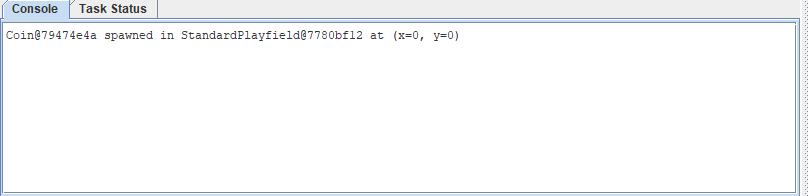
\includegraphics[width=\linewidth]{./figures/console.PNG}
    \end{center}

    In der Konsole siehst du, dass eine Münze (\texttt{Coin}) gespawnt (platziert) wurde. 
    Finde die Koordinaten des Feldes, auf welchem die Münze gespawnt wurde.

    \item Nun suche nach der Stelle im Code der Klasse \lstinline{DemoTask}, in dem die erste Münze erzeugt wird.
    
        Kleiner Tipp: 
        Wenn du \fbox{Strg} drückst wärend du auf einen Klassennamen oder einen Operationsnamen im Code klickst, öffnet Eclipse die entsprechende Java-Datei.
        Alternativ kannst du über den PackageExplorer in das Paket \texttt{de.unistuttagrt.informatik.fius.jvk.tasks} navigieren und dort die Datei \texttt{DemoTask.java} mit einem Doppelklick öffnen.
\end{enumerate}
